\documentclass[10pt,a4paper]{report}
\usepackage[pdftex]{graphicx}
\usepackage{subfigure}            % Multiple figures per float
\usepackage{placeins}             % Fix float loactions with \FloatBarrier
\usepackage{color}                % Color definitions for boxes
\usepackage{multirow}             % Multiple rows per cell in a table
\usepackage{verbatim}             % Long verbatim sections
\usepackage{titlesec}             % Easy modification the chapter format
\usepackage{fancyhdr}             % Easy modification of header and footer
\usepackage{hyperref}			  % Custom hyperlinks

\renewcommand{\arraystretch}{1.2} % Extra space in tables
\parindent0mm                     % New paragraphs start without indentation
\setlength{\parskip}{1em}         % And with a blank line in between

% Redefine chapters to remove the "Chapter" word
\titleformat{\chapter}
  {\normalfont\LARGE\bfseries}{\thechapter}{1em}{}
\titlespacing*{\chapter}{0pt}{3.5ex plus 1ex minus .2ex}{2.3ex plus .2ex}

% Setup hyperlink format in document
\hypersetup{
    colorlinks=true, %set true if you want colored links
    linkcolor=blue,  %choose some color if you want links to stand out
    citecolor=blue,  %choose some color if you want lcitation to stand out
    filecolor=black, % etc...
    urlcolor=blue
}

% Define header and footer
\pagestyle{fancy}
\fancyhf{}
\lhead{C. Rosales}
\rhead{Performance Assessment Workbench User Guide}
\lfoot{PAW User Guide}
\rfoot{\thepage}

% Define header and footer for first page in chapter
\fancypagestyle{plain}{
\fancyhf{}
\lhead{C. Rosales}
\rhead{Performance Assessment Workbench User Guide}
\lfoot{PAW USer Guide}
\rfoot{\thepage}
}

% Gray boxes for optional material
\definecolor{LightGrey}{gray}{.85}
\setlength{\fboxrule}{1pt}
\setlength{\fboxsep}{6pt}
\newcommand{\IntroBox}[1]{
  %\fcolorbox[rgb]{0,0,0}{0.95,0.95,0.95}{
    \fcolorbox{black}{LightGrey}{
    \begin{minipage}{0.94\linewidth}
      %\textbf{Introduction}
      #1
    \end{minipage}
  }
}




\begin{document}

\begin{titlepage}
\thispagestyle{empty}	%don't include number on cover
%\begin{flushleft}
%\begin{figure}
%\includegraphics[width=0.2\textwidth]{gplv3-127x51.png}
%\end{figure}
%\end{flushleft}
\verb+ +
\vspace{1em}
\begin{flushright}
\huge\bf PAW v1.3\\
\rule{\textwidth}{4pt}
\large{\bf Performance Assessment Workbench User Guide\\
Document Revision 1.0\\
\today}
\end{flushright}

%Back of cover page (copyright)
\newpage
\thispagestyle{empty}
\begin{flushleft}
Carlos Rosales Fern\'andez\\
\verb+carlos@tacc.utexas.edu+\\
\vspace{0.5em}
High Performance Computing \\
Texas Advanced Computing Center\\
The University of Texas at Austin\\
\vspace{1cm}
Copyright 2014 Carlos Rosales Fern\'andez and the University of Texas at Austin.
\end{flushleft}
\newpage
\end{titlepage}

\begin{abstract}
The Performance Assessment Workbench (PAW) is an Open Source suite of microbenchmarks designed with simplicity and reliability in mind. This User Guide documents the implementation details and the general usage for all components of PAW. As of version 1.3 the suite contains code designed to test:

\begin{itemize}
\item BLAS floating point performance in CPUs, GPUs and Xeon Phi
\item MPI latency and bandwidth, including point to point and collective calls
\item Data transfer rates between CPU and GPU
\item Data transfer rates between CPU and Xeon Phi coprocessor. 
\end{itemize}

Each of these capabilities is supported by multiple individual codes. Our objective is that each test provided be completely independent of other tests in the suite, so that it can be executed independently of others and its implementation can be reviewed cleanly and without interference.

Excellent microbenchmarks exist already for memory bandwitdth (STREAM, see \cite{stream}), OpenMP overheads (EPCC OMP Benchmark, see \cite{epcc}, and Parallel File System IO (IOR, see \cite{ior}). Together with PAW, these benchmarks provide an excellent starting point for baseline system evaluation.

Throughout the text we have used text boxes to highlight important information. These boxes look like this:

\IntroBox{ These gray boxes contain highlighted material for each section and chapter. }

Our intention is to create a set of simple benchmark implementations that are transparent to use and understand. The hope is that users of this set of tools will actually look at the code implementation and understand exactly what is being measured, without having to peel off multiple layers of obfuscating code. We have made an effort to write simple, reliable, and thoroughly commented C code, but we are well aware that documentation is never perfect or complete. We welcome all feedback. Feedback that includes suggestions for improvement in the usability, reliability, and accuracy of these benchmarks is particularly welcome. 

Version 1.3 is a feature release which adds MPI-3.0 point to point tests to the benchmark suite.
\end{abstract}

\tableofcontents

\chapter{Installation}
The Performance Analysis Workbench is simple to install. In order to use all of its features you will need GNU Make and a C compiler. In order to test GPU performance you will also need the CUDA compiler and CUBLAS linear algebra libraries. If testing the Xeon Phi you will also need a compiler and with support for offload to the Xeon Phi.

First of all obtain the latest version tarball, currently paw-1.3.tar.gz, and expand it in a convenient location in your system:

\begin{verbatim}
    tar xzvf ./paw-1.3.tar.gz
\end{verbatim}

This will create a top level directory called \verb+paw-1.3+, with subdirectories \verb+/bin+, \verb+/doc+, and \verb+/src+. Inside the source directory you will also find separate subdirectories for common functions (\verb+aux+) and the floating point (\verb+/blas+), MPI (\verb+/mpi+), GPU (\verb+/gpu+) and Xeon Phi (\verb+/phi+) benchmarking tools.

Change directory to the top level of PAW and edit \verb+Makefile.in+ to reflect your compiler and library locations. A default template is provided that uses the Intel compiler, the Intel MKL BLAS libraries, the Mvapich2 MPI libraries and NVIDIA's nvcc compiler.

A set of benchmarks for CPU only will be generated using the traditional \texttt{make \&\& make install}. The complete benchmarking suite can be built using:

\begin{verbatim}
    make all
    make all-install
\end{verbatim}

You may also choose to build only a subset of test codes:

\begin{verbatim}
    make blas && make blas-install
    make mpi  && make mpi-install
    make mpi3 && make mpi3-install
    make gpu  && make gpu-install
    make phi  && make phi-install
\end{verbatim}

Notice that the MPI-3.0 tests have been separated from the rest of MPI tests because many libraries still do not support these functions. They may eventually be merged with the rest of the MPI tests.

The executable tests will be placed in the \verb+/bin+ directory unless a \verb+PREFIX=/install/dir/location/+ option is passed to Make in the installation step. For example, to build only the tests relevant to regular CPUs and install the resulting executables in the \verb+/home/me/paw/+ directory one would execute:

\begin{verbatim}
    make blas && make blas-install PREFIX=/home/me/paw
    make mpi  && make mpi-install PREFIX=/home/me/paw
\end{verbatim}

\FloatBarrier
\chapter{General Design}
Each benchmark consists of an innermost loop of count \verb+NLOOP+ that is used to ensure that sufficient time passes between two consecutive timer calls. An outer loop executes \verb+NREPS+ repetitions of the measurement for each workload size, and these runs are used to calculate maximum, minimum, mean, and standard deviation values for the measurement. As the size of the problem increases, the innermost loop iteration count is decreased to avoid excessive runtime, but it is always kept over the safety threshold or over \verb+NLOOP_MIN+ iterations, whichever is more conservative.

Each benchmark will execute the following steps:

\begin{enumerate}
\item Establish timer overhead
\item Determine minimal loop length for timings, \verb+NLOOP+
\begin{itemize}
	\item Run warmup test
	\item Time execution of smallest workload with default \verb+NLOOP+
	\item Reset \verb+NLOOP+ to ensure minimum execution time is 10 times larger than timer overhead
\end{itemize}
\item Execute test for each workload size
\begin{itemize}
	\item Run warmup for this workload
	\item Repeat test \verb+NREPS+ and store timing for each execution
	\item Obtain statistics for test
	\item Write partial results to file
	\item Reset loop length
\end{itemize}

\end{enumerate}

By default the values of \verb+NLOOP+ and \verb+NREPS+ have been set to 1000 and 10 respectively, but one should look carefully at the statistics for each measurement to see if there is a need to increase these.

All constant values controlling iteration and size limits for the microbenchmarks reside in the \texttt{src/aux/constants.h} file, and their use is documented with comments. Changing \verb+NREPS+ requires recompilation of hte suite, but changing the \verb+NLOOP+ iteration limit and the size ranges can be done using environmental variables, as described in Table \ref{tab:env}.

\begin{table}[ht]
\centering
\caption{Environmental variables controlling iteration number and size ranges}
\label{tab:env}
\begin{tabular}{|l|l|l|}
\hline
\bf{Variable}	& \bf{Description}                          & \bf{Default}\\\hline
NLOOP\_MAX      & Number of iterations for each timing run  & 1000\\
NLOOP\_PHI\_MAX & Number of iterations for each Phi timing run  & 100\\
MIN\_BLAS\_SIZE & Minimum size for BLAS tests               & 8\\
MED\_BLAS\_SIZE & Warm up size for BLAS tests               & 1024\\
MAX\_BLAS\_SIZE & Maximum size for BLAS tests               & 10000\\
MIN\_COL\_SIZE  & Minimum size for MPI collective tests     & 1\\
MED\_COL\_SIZE  & Warm up size for MPI collective tests     & 10000\\
MAX\_COL\_SIZE  & Maximum size for MPI collective tests     & 100000\\
MIN\_P2P\_SIZE  & Minimum size for MPI point to point tests & 1\\
MED\_P2P\_SIZE  & Warm up size for MPI point to point tests & 20000\\
MAX\_P2P\_SIZE  & Maximum size for MPI point to point tests & 1000000\\
WINDOW\_SIZE    & Window size for MPI message rate tests    & 128\\
MIN\_GPU\_BLAS\_SIZE & Minimum size for GPU BLAS tests      & 8\\
MED\_GPU\_BLAS\_SIZE & Warm up size for GPU BLAS tests      & 1024\\
MAX\_GPU\_BLAS\_SIZE & Maximum size for GPU BLAS tests      & 9192\\
MIN\_GPU\_SIZE  & Minimum size for GPU data transfer tests  & 128\\
MED\_GPU\_SIZE  & Warm up size for GPU data transfer tests  & 20000\\
MAX\_GPU\_SIZE  & Maximum size for GPU data transfer tests  & 200000000\\
MIN\_PHI\_SIZE  & Minimum size for Phi data transfer tests  & 256\\
MED\_PHI\_SIZE  & Warm up size for Phi data transfer tests  & 8192\\
MAX\_PHI\_SIZE  & Maximum size for Phi data transfer tests  & 614400000\\\hline
\end{tabular}
\end{table}


\FloatBarrier
\chapter{Floating Point Performance}
\label{sec:blas}
\IntroBox{
Floating point performance is the traditional measure of machine performance for High Performance Computing systems, and represents the overall system capability for performing mathematical operations. Typical benchmarks for overall floating point capability are the Linpack benchmark (HPL, used for the TOP500 list, see references \cite{hpl} and \cite{top500}) and matrix matrix multiplication tests. These algebraic tests have highly optimized implementation with high data reuse and fairly limited memory bandwidth requirements, which are capable of achieving floating point performances very close to the theoretical peak performance of the hardware. Floating point performance is critical for scientific workloads, since they very often rely on solving an algebraic system of equations. Even if a scientific workload is not directly solving a system of linear equations it is likely that it will make extensive use of the floating point capability of the system during tasks like post-processing and data analysis. This makes the determination of the floating point capability of a compute system another essential element in an overall understanding of the system performance.}

The tests described in this section are limited to single node executions, since the purpose is to evaluate the processor floating point performance in isolation from network communication and other factors present in distributed execution. Codes are provided to measure the multithreaded performance of the BLAS calls DGEMM, SGEMM, DGEMV and SGEMV using the Intel MKL library or similar.

The code executes each BLAS call within a loop for each matrix size, and the average time is recorded. This loop is repeated \verb+NREPS+ times and the minimum, maximum, and mean values are written to file. The number of iterations in the innermost loop, \verb+NLOOP+, is set dynamically. The code ensures the minimum number of inner loop repetitions is sufficient to obtain an accurate timing for the smallest matrix size. This is done by determining the minimum time that must pass between consecutive timer calls for the measurement to be valid, multiplying this by 10, and using that as the minimum acceptable time that the innermost loop should take. As the size of the problem increases the innermost loop iteration number is decreased to avoid excessive runtime, but it is always kept over the safety threshold or over \verb+NLOOP_MIN+, whichever is most conservative. A warmup execution is run without being timed before each message size is tested.

The setup costs - memory allocation, array initialization, etc - are not considered as part of the timed region. The number of operations required for the matrix matrix multiplication is estimated as $2N^2(N+1)$ for each size $N$, and the number of operations required for the matrix vector multiplication is estimated as $2N(N+1)$ for each size $N$. 

Each test will output two files, \verb+XXXXX_time-np_YYYY.dat+ and \verb+XXXXX_flops-np_YYYY.dat+ with execution timings and floating point operations per second respectively, as well as a brief summary to \verb+stdout+. IN the names the pattern \verb+XXXXX+ corresponds to the blas call name (dgemm, sgemm, dgemv, sgemv) and the pattern \verb+YYYY+ to the number of threads used in the test. Make sure \verb+OMP_NUM_THREADS+ is set to the correct number when you execute these tests, as they rely on this number to write the correct file names.

\FloatBarrier
\chapter{MPI Latency}
\label{sec:latency}
\IntroBox{
MPI latency is of importance to codes that exchange small messages, where latency plays a more significant role than bandwidth. Codes with irregular communication patters typically benefit from short latencies. When looking a latency values off node the limiting factors will be the network interconnect and adapter, while on node the limiting factor will be the memory subsystem, including the socket to socket communication pathways.}

To measure MPI latency we use a round trip of an \verb+MPI_Send+ / \verb+MPI_Recv+ call set. We use a payload of 1 byte only and average the time over \verb+NLOOP+ such exchanges -- after a non-timed warmup exchange. The test is repeated \verb+NREPS+ times, and the results saved to a file called \verb+latency.dat+. A summary of the results is also written to \verb+stdout+. 

The latency code can only be executed between two tasks. An error will be thrown and execution aborted if execution with a different number of MPI tasks is attempted.

\FloatBarrier
\chapter{MPI Bandwidth}
\IntroBox{
Many scientific codes require some type of distributed memory model because of their scale and complexity. The Message Passing Interface (MPI) framework allows for communication in distributed systems, and is the de facto standard for codes working in distributed memory systems. Codes that have large messages to exchange depend heavily on the MPI bandwidth supported by the system for their performance, especially if they execute mainly blocking calls or collective operations. Understanding the achievable MPI bandwidth in a system is critical for estimating scalability of distributed codes.}

The code executes each MPI call (in a ping-pong setup for point to point calls) within a loop of size \verb+NLOOP+ for each message size, and the average time is recorded. This loop is repeated \verb+NREPS+ times and the minimum, maximum, mean and standard deviation values are written to file. A warmup exchange is run without being timed before each message size is tested.

Each MPI task times the exchange, and an \verb+MPI_reduce+ call is used to determine the minimum of the measured times, which is used to calculate the best average time per iteration in the innermost loop. Note that this can cause inaccuracy in the measurements of some collective calls for small messages, as discussed in Section \ref{sec:collectives}.

It is important to note that in the test code task 0 communicates with task n/2, task 1 communicates with task n/2+1, and so on and so forth. This is illustrated in Figure \ref{fig:mpi_test_config} for an example using 16 tasks. This setup must be taken into account for binding purposes, particularly when trying to determine differences between intra socket and inter socket communication, or for inter node communication across different sockets. This pattern has been made the default so that using multiple nodes results in all communications taking place in between nodes rather than within nodes.

\begin{figure}[ht!]
	\centering
	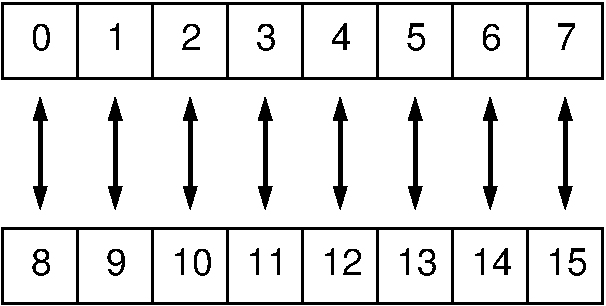
\includegraphics[width=0.5\columnwidth]{figures/mpi_config.pdf}
	\caption{MPI task pairing for point to point communication in a 16 task example.}
	\label{fig:mpi_test_config}
\end{figure}

PAW provides independent codes to measure the performance of the following MPI calls:

\begin{itemize}
\item{Collectives}
\begin{itemize}
    \item{MPI\_Accumulate with active synchronization ( \texttt{col\_acc} )}
    \item{MPI\_Accumulate with passive synchronization ( \texttt{col\_acc\_fence} )}
	\item{MPI\_Allgather ( \texttt{col\_agtr} )}
	\item{MPI\_Allreduce ( \texttt{col\_ardc} )}
	\item{MPI\_Alltoall ( \texttt{col\_a2a} )}
	\item{MPI\_Bcast ( \texttt{col\_bct} )}
	\item{MPI\_Gather ( \texttt{col\_gtr} )}
	\item{MPI\_Reduce ( \texttt{col\_rdc} )}
	\item{MPI\_Raccumulate ( \texttt{col\_racc} )}
	\item{MPI\_Scatter ( \texttt{col\_sct} )}
\end{itemize}
\item{Point to Point}
\begin{itemize}
	\item{MPI\_Get with active synchronization ( \texttt{p2p\_get} )}
	\item{MPI\_Get with passive synchronization ( \texttt{p2p\_get\_fence} )}
	\item{MPI\_Isend ( \texttt{p2p\_isend} )}
	\item{MPI\_Put with active synchronization ( \texttt{p2p\_put} )}
	\item{MPI\_Put with passive synchronization ( \texttt{p2p\_put\_fence} )}
	\item{MPI\_Rget ( \texttt{p2p\_rget} )}
	\item{MPI\_Rput ( \texttt{p2p\_rput} )}
	\item{MPI\_Send ( \texttt{p2p\_send} )}
\end{itemize}
\item{Specialized}
\begin{itemize}
	\item{MPI\_Isend in ping-ping configuration ( \texttt{p2p\_isend\_bidir} )}
	\item{MPI\_Isend using bi-directional communication ( \texttt{p2p\_isend\_ping} )}
	\item{Unidirectional MPI message rate ( \texttt{p2p\_mrate} )}
	\item{Bidirectional MPI message rate ( \texttt{p2p\_mrate\_bidir} )}
\end{itemize}
\end{itemize}

Each of the individual tests is described in the sections below.

\section{MPI-1.0 Collectives}
\label{sec:collectives}

In all collectives tests the call itself is executed by all processes, timed independently, and the minimum value of the timed intervals chosen. Note that this has the serious disadvantage of ignoring issues with messages sent using the eager protocol. An \verb+MPI_Bcast+ or \verb+MPI_Scatter+ using a small message size may report incorrect timings because it is not forced to wait for a completion signal from any of the other tasks involved. This means that the effective bandwidth may be overestimated for small messages in these cases. In order to minimize this effect we use the maximum measured time across all tasks when reporting timings and bandwidth for these two calls, while we use the minimum time for all others. This is not a perfect solution. If precise measurements of the performance of these calls for small messages are required we suggest altering the code to ensure synchronization has completed within the timing section of the code. 

\section{MPI-2.0 Collectives}
\subsection{col\_acc}
The \verb+col_acc+ benchmark uses the \verb+MPI_Accumulate+ call, together with active synchronization calls \verb+MPI_Win_start+, \verb+MPI_Win_complete+, \verb+MPI_Win_post+ and \verb+MPI_Win_wait+. The data is reduced in task 0 using the \verb+MPI_SUM+ operation. Within the timed section of the code only the calls shown in Table \ref{tab:acc} are executed.

\begin{table}[ht]
\centering
\caption{Timed code in \texttt{col\_acc} test.}
\label{tab:acc}
\begin{tabular}{|l|l|}
\hline
\bf{Tasks 1...(n-1)}	   & \bf{Task 0}\\\hline
MPI\_Win\_start( ... );    & MPI\_Win\_post( ... );\\
MPI\_Accumulate( ... );    & MPI\_Win\_wait( ... );\\
MPI\_Win\_complete( ... ); & \\\hline
\end{tabular}
\end{table}

The code writes a summary to \verb+stdout+, and timing and bandwidth results to files named \verb+acc_time-np_XXXX.dat+ and \verb+acc_bw-np_XXXX.dat+, where \verb+XXXX+ is the number of processors used in the test.

\FloatBarrier
\subsection{col\_acc\_fence}
The \verb+col_acc_fence+ benchmark uses the \verb+MPI_Accumulate+ call, together with passive synchronization calls to \verb+MPI_Win_fence+. The data is reduced in task 0 using the \verb+MPI_SUM+ operation. Within the timed section of the code only the calls shown in Table \ref{tab:acc_fence} are executed.

\begin{table}[ht]
\centering
\caption{Timed code in \texttt{col\_acc\_fence} test.}
\label{tab:acc_fence}
\begin{tabular}{|l|l|}
\hline
\bf{Tasks 1...(n-1)}	    & \bf{Task 0}\\\hline
MPI\_Win\_fence( ... ); & MPI\_Win\_fence( ... );\\
MPI\_Accumulate( ... ); & MPI\_Win\_fence( ... );\\
MPI\_Win\_fence( ... ); & \\\hline
\end{tabular}
\end{table}

The code writes a summary to \verb+stdout+, and timing and bandwidth results to files named \verb+accfence_time-np_XXXX.dat+ and \verb+accfence_bw-np_XXXX.dat+, where \verb+XXXX+ is the number of processors used in the test.

\section{MPI-3.0 Collectives}
The \verb+col_racc+ benchmark uses the \verb+MPI_Raccumulate+ call, together with synchronization calls to \verb+MPI_Wait+ (local synchronization), and \verb+MPI_Win_flush_all+ (remote synchronization). The data is reduced in task 0 using the \verb+MPI_SUM+ operation. Within the timed section of the code only the calls shown in Table \ref{tab:racc} are executed.

\begin{table}[ht]
\centering
\caption{Timed code in \texttt{p2p\_racc} test.}
\label{tab:racc}
\begin{tabular}{|l|}
\hline
\bf{Tasks 1...(n-1)}	   \\\hline
MPI\_Raccumulate( ... );           \\
MPI\_Wait( ... );           \\
MPI\_Win\_flush\_all( ... );\\\hline
\end{tabular}
\end{table}

The code writes a summary to \verb+stdout+, and timing and bandwidth results to files named \verb+rget_time-np_XXXX.dat+ and \verb+rget_bw-np_XXXX.dat+, where \verb+XXXX+ is the number of processors used in the test.

\section{MPI-1.0 Point to Point}
This section describes the setup for all MPI-1.0 point to point communication schemes considered in this test suite.

\subsection{p2p\_isend}
The \verb+p2p_isend+ benchmark uses the \verb+MPI_Isend+, \verb+MPI_Irecv+, and \verb+MPI_Wait+ calls. The communication happens in a ping-pong setup, with the first half of the tasks sending data to their partner tasks in the second half, and then reversing the pattern after synchronization. Within the timed section of the code only the calls shown in Table \ref{tab:isend} are executed.

\begin{table}[ht]
\centering
\caption{Timed code in \texttt{p2p\_isend} test.}
\label{tab:isend}
\begin{tabular}{|l|l|}
\hline
\bf{Tasks 0...(n/2-1)}	& \bf{Tasks n/2...(n-1)}\\\hline
MPI\_Isend( ... );      & MPI\_Irecv( ... );\\
MPI\_Wait( ... );       & MPI\_Wait( ... );\\
MPI\_Irecv( ... );      & MPI\_Isend( ... );\\
MPI\_Wait( ... );       & MPI\_Wait( ... );\\\hline
\end{tabular}
\end{table}

The code writes a summary to \verb+stdout+, and timing and bandwidth results to files named \verb+isend_time-np_XXXX.dat+ and \verb+isend_bw-np_XXXX.dat+, where \verb+XXXX+ is the number of processors used in the test.

\FloatBarrier
\subsection{p2p\_send}
The \verb+p2p_isend+ benchmark uses the \verb+MPI_Send+ and \verb+MPI_Recv+ calls. The communication happens in a ping-pong setup, with the first half of the tasks sending data to their partner tasks in the second half, and then reversing the pattern after synchronization. Within the timed section of the code only the calls shown in Table \ref{tab:send} are executed.

\begin{table}[ht]
\centering
\caption{Timed code in \texttt{p2p\_send} test.}
\label{tab:send}
\begin{tabular}{|l|l|}
\hline
\bf{Tasks 0...(n/2-1)}	& \bf{Tasks n/2...(n-1)}\\\hline
MPI\_Send( ... );       & MPI\_Recv( ... );\\
MPI\_Recv( ... );       & MPI\_Send( ... );\\\hline
\end{tabular}
\end{table}

The code writes a summary to \verb+stdout+, and timing and bandwidth results to files named \verb+send_time-np_XXXX.dat+ and \verb+send_bw-np_XXXX.dat+, where \verb+XXXX+ is the number of processors used in the test.

\FloatBarrier
\section{MPI-2.0 Point to Point}
This section describes the setup for all MPI-2.0 point to point communication schemes considered in this test suite.

\subsection{p2p\_get}
The \verb+p2p_get+ benchmark uses the \verb+MPI_Get+ call, together with active synchronization calls \verb+MPI_Win_start+, \verb+MPI_Win_complete+, \verb+MPI_Win_post+ and \verb+MPI_Win_wait+. The communication happens in one direction only, with the first half of the tasks pulling data from their partner tasks in the second half. Within the timed section of the code only the calls shown in Table \ref{tab:get} are executed.

\begin{table}[ht]
\centering
\caption{Timed code in \texttt{p2p\_get} test.}
\label{tab:get}
\begin{tabular}{|l|l|}
\hline
\bf{Tasks 0...(n/2-1)}	   & \bf{Tasks n/2...(n-1)}\\\hline
MPI\_Win\_start( ... );    & MPI\_Win\_post( ... );\\
MPI\_Get( ... );           & MPI\_Win\_wait( ... );\\
MPI\_Win\_complete( ... ); & \\\hline
\end{tabular}
\end{table}

The code writes a summary to \verb+stdout+, and timing and bandwidth results to files named \verb+get_time-np_XXXX.dat+ and \verb+get_bw-np_XXXX.dat+, where \verb+XXXX+ is the number of processors used in the test.

\FloatBarrier
\subsection{p2p\_get\_fence}
The \verb+p2p_get+ benchmark uses the \verb+MPI_Get+ call, together with passive synchronization calls to \verb+MPI_Win_fence+. The communication happens in one direction only, with the first half of the tasks pulling data from their partner tasks in the second half. Within the timed section of the code only the calls shown in Table \ref{tab:get_fence} are executed.

\begin{table}[ht]
\centering
\caption{Timed code in \texttt{p2p\_get\_fence} test.}
\label{tab:get_fence}
\begin{tabular}{|l|l|}
\hline
\bf{Tasks 0...(n/2-1)}	   & \bf{Tasks n/2...(n-1)}\\\hline
MPI\_Win\_fence( ... );    & MPI\_Win\_fence( ... );\\
MPI\_Get( ... );           & MPI\_Win\_fence( ... );\\
MPI\_Win\_fence( ... ); & \\\hline
\end{tabular}
\end{table}

The code writes a summary to \verb+stdout+, and timing and bandwidth results to files named \verb+getfence_time-np_XXXX.dat+ and \verb+getfence_bw-np_XXXX.dat+, where \verb+XXXX+ is the number of processors used in the test.

\FloatBarrier
\subsection{p2p\_put}
The \verb+p2p_put+ benchmark uses the \verb+MPI_Put+ call, together with active synchronization calls \verb+MPI_Win_start+, \verb+MPI_Win_complete+, \verb+MPI_Win_post+ and \verb+MPI_Win_wait+. The communication happens in one direction only, with the first half of the tasks pulling data from their partner tasks in the second half. Within the timed section of the code only the calls shown in Table \ref{tab:put} are executed.

\begin{table}[ht]
\centering
\caption{Timed code in \texttt{p2p\_put} test.}
\label{tab:put}
\begin{tabular}{|l|l|}
\hline
\bf{Tasks 0...(n/2-1)}	   & \bf{Tasks n/2...(n-1)}\\\hline
MPI\_Win\_start( ... );    & MPI\_Win\_post( ... );\\
MPI\_Put( ... );           & MPI\_Win\_wait( ... );\\
MPI\_Win\_complete( ... ); & \\\hline
\end{tabular}
\end{table}

The code writes a summary to \verb+stdout+, and timing and bandwidth results to files named \verb+put_time-np_XXXX.dat+ and \verb+put_bw-np_XXXX.dat+, where \verb+XXXX+ is the number of processors used in the test.

\FloatBarrier
\subsection{p2p\_put\_fence}
The \verb+p2p_put+ benchmark uses the \verb+MPI_Put+ call, together with passive synchronization calls to \verb+MPI_Win_fence+. The communication happens in one direction only, with the first half of the tasks pulling data from their partner tasks in the second half. Within the timed section of the code only the calls shown in Table \ref{tab:put_fence} are executed.

\begin{table}[ht]
\centering
\caption{Timed code in \texttt{p2p\_put\_fence} test.}
\label{tab:put_fence}
\begin{tabular}{|l|l|}
\hline
\bf{Tasks 0...(n/2-1)}	   & \bf{Tasks n/2...(n-1)}\\\hline
MPI\_Win\_fence( ... );    & MPI\_Win\_fence( ... );\\
MPI\_Put( ... );           & MPI\_Win\_fence( ... );\\
MPI\_Win\_fence( ... ); & \\\hline
\end{tabular}
\end{table}

The code writes a summary to \verb+stdout+, and timing and bandwidth results to files named \verb+putfence_time-np_XXXX.dat+ and \verb+putfence_bw-np_XXXX.dat+, where \verb+XXXX+ is the number of processors used in the test.

\FloatBarrier
\section{MPI-3.0 Point to Point}
This section describes the setup for all MPI-3.0 point to point communication schemes considered in this test suite.

\subsection{p2p\_rget}
The \verb+p2p_rget+ benchmark uses the \verb+MPI_Rget+ call, together with synchronization calls to \verb+MPI_Wait+ (local synchronization), and \verb+MPI_Win_flush_all+ (remote synchronization). The communication happens in one direction only, with the first half of the tasks pulling data from their partner tasks in the second half. Within the timed section of the code only the calls shown in Table \ref{tab:rget} are executed.

\begin{table}[ht]
\centering
\caption{Timed code in \texttt{p2p\_rget} test.}
\label{tab:rget}
\begin{tabular}{|l|}
\hline
\bf{Tasks 0...(n/2-1)}	   \\\hline
MPI\_Rget( ... );           \\
MPI\_Wait( ... );           \\
MPI\_Win\_flush\_all( ... );\\\hline
\end{tabular}
\end{table}

The code writes a summary to \verb+stdout+, and timing and bandwidth results to files named \verb+rget_time-np_XXXX.dat+ and \verb+rget_bw-np_XXXX.dat+, where \verb+XXXX+ is the number of processors used in the test.

\FloatBarrier
\subsection{p2p\_rput}
The \verb+p2p_rput+ benchmark uses the \verb+MPI_Rput+ call, together with synchronization calls \verb+MPI_Win_wait+ (local synchronization) and \verb+MPI_Win_flush_all+ (remote synchronization). The communication happens in one direction only, with the first half of the tasks pulling data from their partner tasks in the second half. Within the timed section of the code only the calls shown in Table \ref{tab:rput} are executed.

\begin{table}[ht]
\centering
\caption{Timed code in \texttt{p2p\_rput} test.}
\label{tab:rput}
\begin{tabular}{|l|}
\hline
\bf{Tasks 0...(n/2-1)} \\\hline
MPI\_Rput( ... );      \\
MPI\_Wait( ... );      \\
MPI\_Win\_flush\_all( ... );\\\hline
\end{tabular}
\end{table}

The code writes a summary to \verb+stdout+, and timing and bandwidth results to files named \verb+put_time-np_XXXX.dat+ and \verb+put_bw-np_XXXX.dat+, where \verb+XXXX+ is the number of processors used in the test.

\section{Specialized}
This section describes point to point measurements that do not employ a ping-pong setup, and that are used for specialized purposes.

\FloatBarrier
\subsection{p2p\_isend\_bidir}
Some high performance interconnects will allow for simultaneous bidirectional traffic, potentially doubling the effective network bandwidth. This test uses non-blocking MPI calls \verb+MPI_Isend+ and \verb+MPI_Irecv+ completed by \verb+MPI_Waitall+ statements. 
Within the timed section of the code only the calls shown in Table \ref{tab:bidir} are executed.

\begin{table}[ht]
\centering
\caption{Timed code in \texttt{p2p\_isend\_bidir} test.}
\label{tab:bidir}
\begin{tabular}{|l|l|}
\hline
\bf{Tasks 0...(n/2-1)}	& \bf{Tasks n/2...(n-1)}\\\hline
MPI\_Isend( ... );      & MPI\_Irecv( ... );\\
MPI\_Irecv( ... );      & MPI\_Isend( ... );\\
MPI\_Waitall( ... );    & MPI\_Waitall( ... )\\\hline
\end{tabular}
\end{table}

The code writes a summary to \verb+stdout+, and timing and bandwidth results to files named \verb+isend_bidir_time-np_XXXX.dat+ and \verb+isend_bidir_bw-np_XXXX.dat+, where \verb+XXXX+ is the number of processors used in the test.

\FloatBarrier
\subsection{p2p\_isend\_ping}
The \verb+p2p_isend_ping+ benchmark uses the \verb+MPI_Isend+, \verb+MPI_Irecv+, and \verb+MPI_Wait+ calls. The communication happens in a ping-ping setup, with the first half of the tasks sending data to their partner tasks in the second half. This setup is useful in order to measure asymmetries in the exchange, which would be averaged out by a ping-pong setup. While no asymmetries are expected between identical devices this test can be useful when exchagning data between two different processor types, or between a traditional processor and a coprocessor or accelerator device. Within the timed section of the code only the calls shown in Table \ref{tab:ping} are executed.

\begin{table}[ht]
\centering
\caption{Timed code in \texttt{p2p\_isend} test.}
\label{tab:ping}
\begin{tabular}{|l|l|}
\hline
\bf{Tasks 0...(n/2-1)}	& \bf{Tasks n/2...(n-1)}\\\hline
MPI\_Isend( ... );      & MPI\_Irecv( ... );\\
MPI\_Wait( ... );       & MPI\_Wait( ... );\\
MPI\_Irecv( ... );      & MPI\_Isend( ... );\\
MPI\_Wait( ... );       & MPI\_Wait( ... );\\\hline
\end{tabular}
\end{table}

The code writes a summary to \verb+stdout+, and timing and bandwidth results to files named \verb+isend_ping_time-np_XXXX.dat+ and \verb+isend_ping_bw-np_XXXX.dat+, where \verb+XXXX+ is the number of processors used in the test.

\FloatBarrier

\subsection{p2p\_mrate}
The \verb+p2p_mrate+ benchmark uses the \verb+MPI_Isend+, \verb+MPI_Irecv+, and \verb+MPI_Waitall+ calls. The communication happens in a pipelined ping-ping setup, with the first half of the tasks sending data to their partner tasks in the second half. A user given window size determines how many messages are pipelined one after another before performing a synchronization call, with the aim of determining the sustained message rate of the network. This number is defined in the file \verb+src/aux/constants.h+ as \verb+DEFAULT_WINDOW_SIZE+ but can be overwritten using the environmental variable \verb+WINDOW_SIZE+  Within the timed section of the code only the calls shown in Table \ref{tab:mrate} are executed, with WS standing for the window size value.

\begin{table}[ht]
\centering
\caption{Timed code in \texttt{p2p\_mrate} test.}
\label{tab:mrate}
\begin{tabular}{|l|l|}
\hline
\bf{Tasks 0...(n/2-1)}	& \bf{Tasks n/2...(n-1)}\\\hline
for(k=0;k$<$WS;k++)\{     & for(k=0;k$<$WS;k++)\{ \\
\verb+    +MPI\_Isend( ... );      & \verb+    +MPI\_Irecv( ... );\\
\}MPI\_Waitall(...);    & \}MPI\_Waitall(...);\\\hline
\end{tabular}
\end{table}

The code writes a summary to \verb+stdout+, and timing and bandwidth results to files named \verb+mrate_time-np_XXXX.dat+ and \verb+mrate_rate-np_XXXX.dat+, where \verb+XXXX+ is the number of processors used in the test.

\FloatBarrier

\subsection{p2p\_mrate\_bidir}
The \verb+p2p_mrate_bidir+ benchmark uses the \verb+MPI_Isend+, \verb+MPI_Irecv+, and \verb+MPI_Waitall+ calls. The communication happens in a pipelined bidirectional ping-ping setup, with all tasks sending data to and receiving data from their partner tasks. A user given window size determines how many messages are pipelined one after another before performing a synchronization call, with the aim of determining the sustained message rate of the network. This number is defined in the file \verb+src/aux/constants.h+ as \verb+DEFAULT_WINDOW_SIZE+ but can be overwritten using the environmental variable \verb+WINDOW_SIZE+  Within the timed section of the code only the calls shown in Table \ref{tab:mrate_bdr} are executed, with WS standing for the window size value.

\begin{table}[ht]
\centering
\caption{Timed code in \texttt{p2p\_mrate} test.}
\label{tab:mrate_bdr}
\begin{tabular}{|l|l|}
\hline
\bf{Tasks 0...(n/2-1)}	      & \bf{Tasks n/2...(n-1)}\\\hline
for(k=0;k$<$WS;k++)\{          & for(k=0;k$<$WS;k++)\{ \\
\verb+    +MPI\_Isend( ... );  & \verb+    +MPI\_Irecv( ... );\\
\verb+    +MPI\_Irecv( ... );  & \verb+    +MPI\_Isend( ... );\\
\}MPI\_Waitall(...);    & \}MPI\_Waitall(...);\\\hline
\end{tabular}
\end{table}

The code writes a summary to \verb+stdout+, and timing and bandwidth results to files named \verb+mrate_bidir_time-np_XXXX.dat+ and \verb+mrate_bidir_rate-np_XXXX.dat+, where \verb+XXXX+ is the number of processors used in the test.

\FloatBarrier
\chapter{GPU}
GPUs can provide a high theoretical peak performance, but can be limited in their usability due to data transfer bottlenecks across the PCIe bus. This makes important the measurement of data transfer rates between CPU and GPU. This section provides a description of the tests for floating point performance and data transfer rates for GPUs (using NVIDIA's CUDA) provided with PAW.

\section{Floating Point Performance}
\label{sec:gpu_fp}
GPUs traditionally provide a high theoretical peak rate, by including a large number of simple processing units that, on aggregate, yield impressive floating point performance.

PAW provides code designed to test DGEMM and SGEMM calls from the cublas library. As with all PAW benchmarks the timer overhead is taken into account when defining the minimum number of iterations to execute for the smallest workload to be measured, and \verb+NLOOP+ is then dynamically adjusted to avoid spending too much time testing a particular workload size. A warmup call is performed outside the timed loop for every workload size. Each size is tested \verb+NREPS+ times in order to gather statistics for the timings.

It is important to mention that the \verb+cublasSetVector+ calls used to transfer data to the GPU are not timed as part of this measurement. Only the execution of the \verb+cublasDgemm+ and \verb+cublasSgemm+ calls is actually timed. It would be simple to change the code to include these into the timed section if necessary.

The two executables are simply called \verb+gpu_dgemm+ and \verb+gpu_sgemm+


\section{Data Transfer Rates}
\label{sec:gpu_bw}
To measure the data transfer to and from the GPU a setup similar to that used for measuring MPI data transfers was used. The device memory is allocated with a \verb+cudaMalloc+ call, and the transfer performed using \verb+cudaMemcpy+. Multiple messages are sent within a timed loop, and the average value is taken. A warmup message is exchanged outside the timed section of the code, before the loop starts. This measurement is run \verb+NREPS+ times and the maximum, minimum and mean values are stored to a file for each message size. As in the MPI bandwidth measurements, care is taken to set the inner loop count to a value such that an accurate timing can be obtained even for the smallest message exchanged. In the cases where pinned memory is used the \verb+cudaMallocHost+ call is used to allocate the host side array.

Several variants of the tests are provided: single direction exchange, round trip, pinned memory and non pinned memory. Table \ref{tab:gpu_bw} describes all variants of the test included with PAW.

\begin{table}[ht]
\centering
\caption{Tests for GPU Data Transfer Rates}
\label{tab:gpu_bw}
\begin{tabular}{|l|l|l|}
\hline
\bf{Name}	                & \bf{Direction}          & \bf{Memory}\\\hline
\texttt{gpu\_in\_pinned}    & CPU to GPU              & Pinned\\
\texttt{gpu\_inout\_pinned} & CPU to GPU + GPU to CPU & Pinned\\
\texttt{gpu\_out\_pinned}   & GPU to CPU              & Pinned\\
\texttt{gpu\_in\_nopin}     & CPU to GPU              & Not Pinned\\
\texttt{gpu\_inout\_nopin}  & CPU to GPU + GPU to CPU & Not Pinned\\
\texttt{gpu\_out\_nopin}    & GPU to CPU              & Not Pinned\\
\hline
\end{tabular}
\end{table}


\FloatBarrier
\chapter{Xeon Phi}
\IntroBox{
The Intel Xeon Phi is a coprocessor that takes advantage of vectorizable threaded codes to provide high floating point rates. While the Xeon Phi runs its own Operating System, and has a much more flexible execution mode than a GPU, it is still connected to the host CPU by the PCI Express bus, and that can result in a communication bottleneck when large amounts of data must be exchanged often between the two, just like in the case of GPU-enabled codes. One could argue that in this case the CPU could be taken out of the equation, since code can be executed natively on the Xeon Phi, but given the limited amount of on-board memory present on the device most codes will utilize several Phis or multiple Phis and host CPUs. This makes it important to look at data transfer rates between CPU and MIC, as it was done for GPUs.}

\section{Data Transfer Rates}
\label{sec:phi_bw}
Several factors affect the speed of an offload data transfer to the MIC. By default, when data is transfered to the MIC as part of an offload region, the runtime will allocate memory on the coprocessor, copy the data over, operate on it as needed, transfer it back to the host, and free memory on the coprocessor. Sometimes this is exactly the behavior required by the code but other times it is OK to maintain the allocated memory on the MIC without freeing it on return, and treat it as persistent in the same way that a CUDA memory transfer works for a GPU. The overhead of allocation and deallocation can be particularly noticeable when performing an offload inside a loop. Another issue that could affect data transfers is data alignment. Last, but not least, message size will be important as well.

Several tests are provided to evaluate data transfers considering all these variables. Table \ref{tab:phi_bw} describes all available tests in PAW.

\begin{table}[ht]
\centering
\caption{Tests for Phi Data Transfer Rates}
\label{tab:phi_bw}
\begin{tabular}{|l|l|l|l|}
\hline
\bf{Name}	                     & \bf{Direction}          & \bf{Reallocate?} & \bf{Memory}\\\hline
\texttt{phi\_alloc\_al\_in}      & CPU to PHI              & YES & Aligned\\
\texttt{phi\_alloc\_al\_inout}   & CPU to PHI + PHI to CPU & YES & Aligned\\
\texttt{phi\_alloc\_al\_out}     & PHI to CPU              & YES & Aligned\\
\texttt{phi\_alloc\_noal\_in}    & CPU to PHI              & YES & Not Aligned\\
\texttt{phi\_alloc\_noal\_inout} & CPU to PHI + PHI to CPU & YES & Not Aligned\\
\texttt{phi\_alloc\_noal\_out}   & PHI to CPU              & YES & Not Aligned\\
\texttt{phi\_keep\_al\_in}       & CPU to PHI              & NO  & Aligned\\
\texttt{phi\_keep\_al\_inout}    & CPU to PHI + PHI to CPU & NO  & Aligned\\
\texttt{phi\_keep\_al\_out}      & PHI to CPU              & NO  & Aligned\\
\texttt{phi\_keep\_noal\_in}     & CPU to PHI              & NO  & Not Aligned\\
\texttt{phi\_keep\_noal\_inout}  & CPU to PHI + PHI to CPU & NO  & Not Aligned\\
\texttt{phi\_keep\_noal\_out}    & PHI to CPU              & NO  & Not Aligned\\
\hline
\end{tabular}
\end{table}

\FloatBarrier
\subsection{Dual Phi Systems}
In order to investigate the effective transfer rates in dual mic nodes two individual offload tests are executed simultaneously, one to device \verb+mic:0+ and one to device \verb+mic:1+. The code uses two OpenMP threads that execute, independently from each other, an offload from thread 0 to mic:0 and an offload from thread 1 to mic:1. Keep in mind that this design is not perfect, and allows for transfers that do not overlap for 100\% of the transference time. However, given the simplicity of the test, it is unlikely that the offloads are started with a significant delay with respect to one another. This test also happens to  reproduce fairly well a situation that one may expect in a real application code, and we believe the information it provides is relevant and useful. 

Every test in Table \ref{tab:phi_bw} will automatically detect the presence of multiple Phi devices and run this additional test if needed. Output files from these dual Phi tests will be saved with a \verb|_mic0+1| suffix to differentiate them from the single Phi tests. 

\FloatBarrier
\addcontentsline{toc}{section}{\bf References}
\begin{thebibliography}{00}

\bibitem{stream}STREAM is the industry standard memory bandwidth benchmark, created by John D. McCalpin.  For more information visit the official STREAM benchmark web site: \href{http://www.cs.virginia.edu/stream/}{www.cs.virginia.edu/stream/}

\bibitem{epcc} The EPCC OpenMP micro-benchmark suite is designed to measure overheads of synchronization, loop scheduling and array operations in the OpenMP runtime library. For more information visit the official EPCC benchmarking website:  \href{http://www.epcc.ed.ac.uk/research/computing/performance-characterisation-and-benchmarking/}{\small www.epcc.ed.ac.uk/research/computing/performance-characterisation-and-benchmarking/}

\bibitem{ior} The IOR benchmark is designed to measure IO performance at the  POSIX and MPI-IO level. For more information visit: \href{http://github.com/chaos/ior/}{github.com/chaos/ior/}

\bibitem{hpl} J. Dongarra, The LINPACK Benchmark: An Explanation, \textit{Proceedings of the 1st International Conference on Supercomputing}, 456--474 (1988)

\bibitem{top500} The TOP500 list ranks commercially available supercomputers in order of performance, as measured by executing the High Performance Linpack (HPL) benchmark. For more information see: \href{http://www.top500.org/}{www.top500.org/}

\end{thebibliography}

\end{document}
